\chapter{Results}
As discussed in chapter \ref{chap:method} the PD algorithm was initially tuned to make sure that the states ($\phi, \theta, z$) were stable on their own. This was done by giving the vehicle a fixed thrust in the $x$ direction, which resulted in the following proportional and derivative gains
\begin{align}
    K_{p} & = 1 \\
    K_{d} & = 0.1
\end{align}
In order to sufficiently train the DDPG algorithm the simulation was executed over $N = 400$ episodes, where each episode consisted of $t = [1, T=1000]$ steps. For each episode the algorithm will therefore be executed until T = 1000 \mathbf{or} the BlueROV2 reaches the terminal state, indicating the it has reached the desired position and orientation. The reward discount factor $\gamma$, learning rate for the actor network $\alpha_{a}$, learning rate for the critic network $\alpha_{q}$ and the exploitation/exploration factor $\epsilon$ were initially defined as
\begin{align}
    \gamma & = 0.9 \\
    \alha_{a} & = 1e-4 \\
    \alpha_{q} & = 1e-4 \\
    \epsilon & = 1
\end{align}
Recall $\alpha_{a}, \alpha_{q}$ and $\epsilon$ should all decrease over the number of iteration, since the algorithm gains larger and larger knowledge about the environment. This was by discounting the parameters at each episode, $N$.\\\\
To accomplish Station Keeping the desired positions and orientations were defined as
\begin{align}
    s_{d} & = [x_{d}, y_{d}, \psi_{d}] = [1, 1, 0] \\
    s_{d,PD} & = [z_{d}, \phi_{d}, \theta_{d}] = [0, 0, 0]
\end{align}
Meaning that the BlueROV2 should stabilise at [$x = 1, y = 1$] in (NED).  
\section{Simulation 1}
As mentioned in chapter \ref{chap:method}, the reward function design is critical for the performance of the algorithm. Initially the reward function was defined with respect to the BlueROV2s' distance to the desired state, meaning that a larger distance should give a lower reward. The reward function, $r(s_{t}, a_{t})$, was therefore defined as
\begin{align}
    r(s_{t}, a_{t}) & = \frac{1}{\norm{s_{e}}} \\
    s_{e} & = s_{d} - s_{t} \\
    R_{N_{i}} & += r(s_{t}, a_{t})
\end{align}
where $R_{N_{i}}$ is the total reward over episode $N_{i}$, where $i=1,..,N$. Because of uncertainty in the measurements a vector consisting of the mean value over the 100 latest total rewards, $[R_{N_{i-100}},...,R_{N_{i}}]$, was defined. By plotting this vector over $N$ episodes the following result was obtained
\begin{figure}[H]
    \centering
    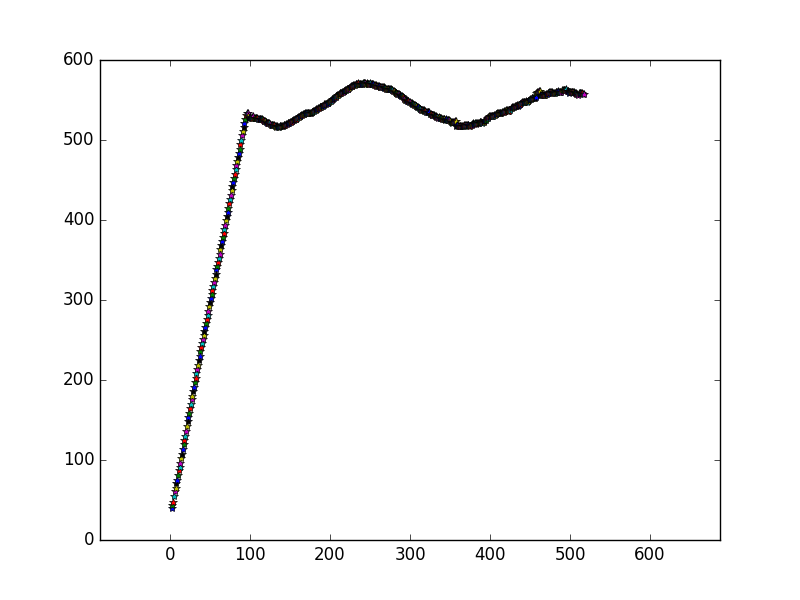
\includegraphics[width=0.7\textwidth]{images/chap5/figure_1.png}
    \caption{Simulation 1}
    \label{fig:sim1}
\end{figure}
In figure \ref{fig:sim1} the $y-axis$ specifies the total reward, and the $x-axis$ specifies number of episode. From the figure we see that the total reward converges to an oscillating value. Since the figure displays the mean value over the 100 latest episodes it is expected that the graph converges to a constant value, because the algorithm should learn the optimal action to take in every state, which results in the total reward being constant in each episode after it has learned the optimal behaviour. However, as previously stated the episodes is defined in such a way that the algorithm will be executed until T = 1000, or the BlueROV2 reaches the terminal state. This means that although it receives the highest reward at the desired position the episode will also terminate at this position, meaning that it will receive a larger total reward, $R_{N}$, by circulating the desired pose for $t=[1,T]$. This shows the importance of the reward function design, since the algorithm is able to find the optimal policy in each state, but the framework defined by the reward function is not optimal. 
\section{Simulation 2}
From the knowledge gained in simulation 1 it was clear that the reward function needed to be redesigned, in order to compensate for the fact that the algorithm received larger rewards for circulating the desired pose compared to reaching the terminal state. The new reward function was therefore defined as

\begin{algorithm}[H]
\SetAlgoLined
\begin{align}
    r(s_{t}, a_{t}) & = \frac{1}{\norm{s_{e}}} \\
    r(s_{t}, a_{t}) & += -0.05*t
\end{align}
    \If{abs($s_{e}$[0]) $<$ 0.1 \textbf{and} abs($s_{e}$[1]) $<$ 0.1}{
    r += 20 \\
    done = \textbf{True}
    }
    \If{$s_{e, diff}$[0] $<$ 0 \textbf{and} abs($s_{e, diff}$[1]) $<$ 0}{
    r += -5
    }
\caption{Reward function}
\label{alg:reward_func}
\end{algorithm}
The algorithm now receives a negative reward, or a penalty, at each step $t$, meaning that it accomplishes the greatest total reward when reaching the desired pose using minimum steps. This will therefore prevent circulating the desired pose being the optimal behaviour. In algorithm \ref{alg:reward_func} I have included two if-sentences, where the first one checks the absolute error in the $x-$ and $y$ position. The reason for neglecting the error in $\psi$ here is that this state is valued less than the other two states. For Station Keeping the $x-$ and $y$ positions are more "\textit{relevant}". The second if-sentence evaluates $s_{e,diff}$, which is defined as the difference between the current error values and the error values in the previous step, $t-1$. If this difference is negative it means that the AUV moves away from the desired pose, which results in an additional penalty. 
\begin{figure}[H]
    \centering
    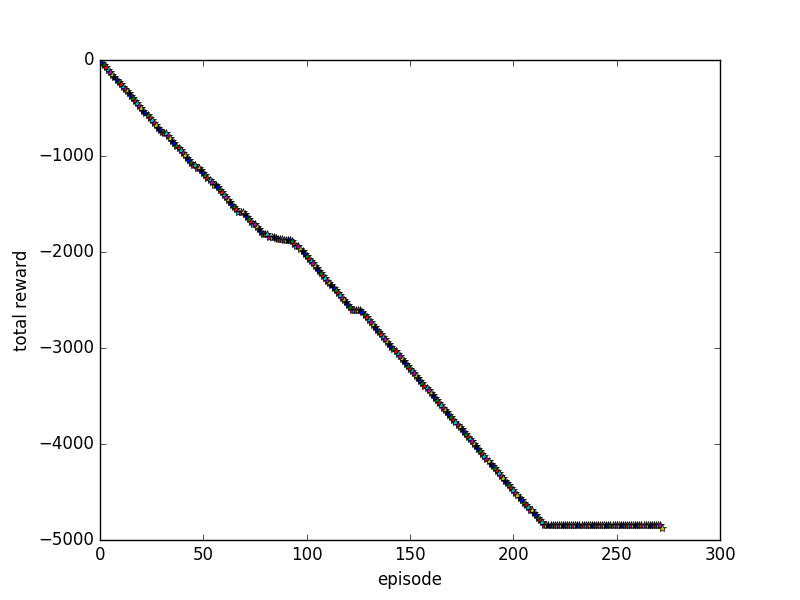
\includegraphics[width=0.7\textwidth]{images/chap5/figure_1-1.png}
    \caption{Simulation 2}
    \label{fig:sim2}
\end{figure}
The result from simulation 2 is illustrated in figure \ref{fig:sim2}. Here we see that the algorithm converges to a constant total reward of $\approx$ -4800 after $\approx$ 215 episodes. Compared to simulation 1 the oscillating behaviour is removed, and the algorithm has successfully learned the optimal behaviour for Station Keeping at the desired pose. 